\PassOptionsToPackage{unicode=true}{hyperref} % options for packages loaded elsewhere
\PassOptionsToPackage{hyphens}{url}
%
\documentclass[12pt,ignorenonframetext,aspectratio=169]{beamer}
\usepackage{pgfpages}
\setbeamertemplate{caption}[numbered]
\setbeamertemplate{caption label separator}{: }
\setbeamercolor{caption name}{fg=normal text.fg}
\beamertemplatenavigationsymbolsempty
% Prevent slide breaks in the middle of a paragraph:
\widowpenalties 1 10000
\raggedbottom
\setbeamertemplate{part page}{
\centering
\begin{beamercolorbox}[sep=16pt,center]{part title}
  \usebeamerfont{part title}\insertpart\par
\end{beamercolorbox}
}
\setbeamertemplate{section page}{
\centering
\begin{beamercolorbox}[sep=12pt,center]{part title}
  \usebeamerfont{section title}\insertsection\par
\end{beamercolorbox}
}
\setbeamertemplate{subsection page}{
\centering
\begin{beamercolorbox}[sep=8pt,center]{part title}
  \usebeamerfont{subsection title}\insertsubsection\par
\end{beamercolorbox}
}
\AtBeginPart{
  \frame{\partpage}
}
\AtBeginSection{
  \ifbibliography
  \else
    \frame{\sectionpage}
  \fi
}
\AtBeginSubsection{
  \frame{\subsectionpage}
}
\usepackage{lmodern}
\usepackage{amssymb,amsmath}
\usepackage{ifxetex,ifluatex}
\usepackage{fixltx2e} % provides \textsubscript
\ifnum 0\ifxetex 1\fi\ifluatex 1\fi=0 % if pdftex
  \usepackage[T1]{fontenc}
  \usepackage[utf8]{inputenc}
  \usepackage{textcomp} % provides euro and other symbols
\else % if luatex or xelatex
  \usepackage{unicode-math}
  \defaultfontfeatures{Ligatures=TeX,Scale=MatchLowercase}
\fi
\usetheme[]{metropolis}
% use upquote if available, for straight quotes in verbatim environments
\IfFileExists{upquote.sty}{\usepackage{upquote}}{}
% use microtype if available
\IfFileExists{microtype.sty}{%
\usepackage[]{microtype}
\UseMicrotypeSet[protrusion]{basicmath} % disable protrusion for tt fonts
}{}
\IfFileExists{parskip.sty}{%
\usepackage{parskip}
}{% else
\setlength{\parindent}{0pt}
\setlength{\parskip}{6pt plus 2pt minus 1pt}
}
\usepackage{hyperref}
\hypersetup{
            pdftitle={Bayesian regression models},
            pdfauthor={Bruno Nicenboim / Shravan Vasishth},
            pdfborder={0 0 0},
            breaklinks=true}
\urlstyle{same}  % don't use monospace font for urls
\newif\ifbibliography
\usepackage{color}
\usepackage{fancyvrb}
\newcommand{\VerbBar}{|}
\newcommand{\VERB}{\Verb[commandchars=\\\{\}]}
\DefineVerbatimEnvironment{Highlighting}{Verbatim}{commandchars=\\\{\}}
% Add ',fontsize=\small' for more characters per line
\usepackage{framed}
\definecolor{shadecolor}{RGB}{248,248,248}
\newenvironment{Shaded}{\begin{snugshade}}{\end{snugshade}}
\newcommand{\AlertTok}[1]{\textcolor[rgb]{0.94,0.16,0.16}{#1}}
\newcommand{\AnnotationTok}[1]{\textcolor[rgb]{0.56,0.35,0.01}{\textbf{\textit{#1}}}}
\newcommand{\AttributeTok}[1]{\textcolor[rgb]{0.77,0.63,0.00}{#1}}
\newcommand{\BaseNTok}[1]{\textcolor[rgb]{0.00,0.00,0.81}{#1}}
\newcommand{\BuiltInTok}[1]{#1}
\newcommand{\CharTok}[1]{\textcolor[rgb]{0.31,0.60,0.02}{#1}}
\newcommand{\CommentTok}[1]{\textcolor[rgb]{0.56,0.35,0.01}{\textit{#1}}}
\newcommand{\CommentVarTok}[1]{\textcolor[rgb]{0.56,0.35,0.01}{\textbf{\textit{#1}}}}
\newcommand{\ConstantTok}[1]{\textcolor[rgb]{0.00,0.00,0.00}{#1}}
\newcommand{\ControlFlowTok}[1]{\textcolor[rgb]{0.13,0.29,0.53}{\textbf{#1}}}
\newcommand{\DataTypeTok}[1]{\textcolor[rgb]{0.13,0.29,0.53}{#1}}
\newcommand{\DecValTok}[1]{\textcolor[rgb]{0.00,0.00,0.81}{#1}}
\newcommand{\DocumentationTok}[1]{\textcolor[rgb]{0.56,0.35,0.01}{\textbf{\textit{#1}}}}
\newcommand{\ErrorTok}[1]{\textcolor[rgb]{0.64,0.00,0.00}{\textbf{#1}}}
\newcommand{\ExtensionTok}[1]{#1}
\newcommand{\FloatTok}[1]{\textcolor[rgb]{0.00,0.00,0.81}{#1}}
\newcommand{\FunctionTok}[1]{\textcolor[rgb]{0.00,0.00,0.00}{#1}}
\newcommand{\ImportTok}[1]{#1}
\newcommand{\InformationTok}[1]{\textcolor[rgb]{0.56,0.35,0.01}{\textbf{\textit{#1}}}}
\newcommand{\KeywordTok}[1]{\textcolor[rgb]{0.13,0.29,0.53}{\textbf{#1}}}
\newcommand{\NormalTok}[1]{#1}
\newcommand{\OperatorTok}[1]{\textcolor[rgb]{0.81,0.36,0.00}{\textbf{#1}}}
\newcommand{\OtherTok}[1]{\textcolor[rgb]{0.56,0.35,0.01}{#1}}
\newcommand{\PreprocessorTok}[1]{\textcolor[rgb]{0.56,0.35,0.01}{\textit{#1}}}
\newcommand{\RegionMarkerTok}[1]{#1}
\newcommand{\SpecialCharTok}[1]{\textcolor[rgb]{0.00,0.00,0.00}{#1}}
\newcommand{\SpecialStringTok}[1]{\textcolor[rgb]{0.31,0.60,0.02}{#1}}
\newcommand{\StringTok}[1]{\textcolor[rgb]{0.31,0.60,0.02}{#1}}
\newcommand{\VariableTok}[1]{\textcolor[rgb]{0.00,0.00,0.00}{#1}}
\newcommand{\VerbatimStringTok}[1]{\textcolor[rgb]{0.31,0.60,0.02}{#1}}
\newcommand{\WarningTok}[1]{\textcolor[rgb]{0.56,0.35,0.01}{\textbf{\textit{#1}}}}
\usepackage{longtable,booktabs}
\usepackage{caption}
% These lines are needed to make table captions work with longtable:
\makeatletter
\def\fnum@table{\tablename~\thetable}
\makeatother
\usepackage{graphicx,grffile}
\makeatletter
\def\maxwidth{\ifdim\Gin@nat@width>\linewidth\linewidth\else\Gin@nat@width\fi}
\def\maxheight{\ifdim\Gin@nat@height>\textheight\textheight\else\Gin@nat@height\fi}
\makeatother
% Scale images if necessary, so that they will not overflow the page
% margins by default, and it is still possible to overwrite the defaults
% using explicit options in \includegraphics[width, height, ...]{}
\setkeys{Gin}{width=\maxwidth,height=\maxheight,keepaspectratio}
\setlength{\emergencystretch}{3em}  % prevent overfull lines
\providecommand{\tightlist}{%
  \setlength{\itemsep}{0pt}\setlength{\parskip}{0pt}}
\setcounter{secnumdepth}{5}

% set default figure placement to htbp
\makeatletter
\def\fps@figure{htbp}
\makeatother

  \setbeamercolor{frametitle}{bg=gray}
  \hypersetup{colorlinks,citecolor=orange,filecolor=red,linkcolor=brown,urlcolor=blue}
% \setsansfont[BoldFont={FiraSans-Bold.ttf}]{FiraSans-Light.ttf}
% \setmonofont{FiraMono-Regular.ttf}
\usepackage[sfdefault]{FiraSans}
\newcommand{\hideFromPandoc}[1]{#1}
         \hideFromPandoc{
             \let\Begin\begin
             \let\End\end
         }

\setbeamerfont{caption}{size=\scriptsize}

\title{Bayesian regression models}
\author{Bruno Nicenboim / Shravan Vasishth}
\date{2020-03-12}

\begin{document}
\frame{\titlepage}

\begin{frame}
\tableofcontents[hideallsubsections]
\end{frame}
\hypertarget{sec:pupil}{%
\section{A first linear model: Does attentional load affect pupil size?}\label{sec:pupil}}

\small

\normalsize

\begin{frame}

\begin{block}{Data:}

One participant's pupil size of the control experiment of Wahn et al. (2016) averaged by trial

\end{block}

\begin{block}{Task:}

A participant covertly tracked between zero and five objects among several randomly moving objects on a computer screen; multiple object tracking--MOT-- (Pylyshyn and Storm 1988) task

\end{block}

\begin{block}{Research question:}

How does the number of moving objects being tracked (attentional load) affect pupil size?

\end{block}

\end{frame}

\begin{frame}



\small

\begin{figure}

{\centering 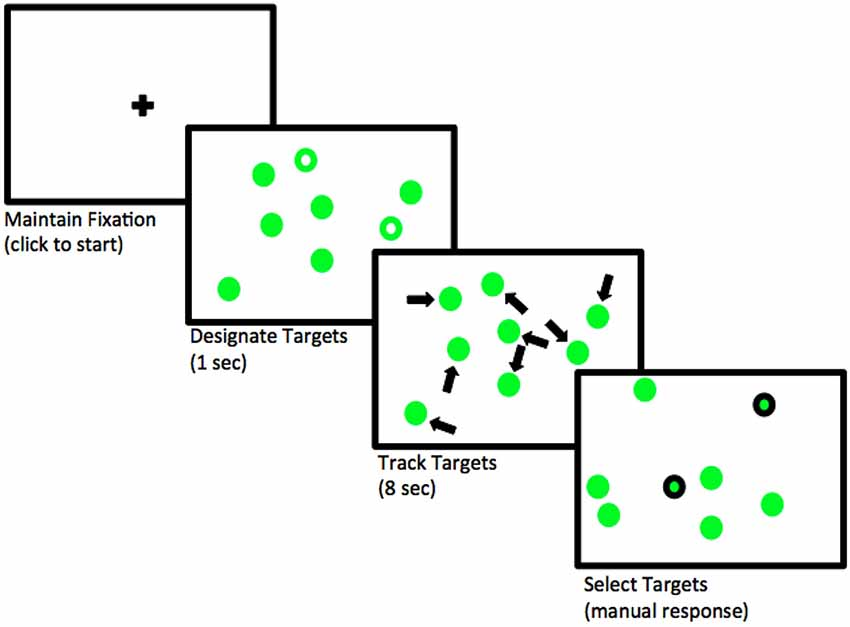
\includegraphics[width=0.8\linewidth]{cc_figure/MOT} 

}

\caption{Flow of events in a trial where two objects needs to be tracked. Adapted from Blumberg, Peterson, and Parasuraman (2015); licensed under CC BY 4.0.}\label{fig:mot}
\end{figure}

\normalsize

\end{frame}

\begin{frame}

\begin{block}{Assumptions:}

\begin{enumerate}
\tightlist
\item
  There is some average pupil size represented by \(\alpha\).
\item
  The increase of attentional load has a linear relationship with pupil size, determined by \(\beta\).
\item
  There is some noise in this process, that is, variability around the true pupil size i.e., a scale, \(\sigma\).
\item
  The noise is normally distributed.
\end{enumerate}

\end{block}

\end{frame}

\begin{frame}{Formal model}
\protect\hypertarget{formal-model}{}

\begin{block}{Likelihood for each observation \(n\):}

\begin{equation}
p\_size_n \sim Normal(\alpha + c\_load_n \cdot \beta,\sigma)
\end{equation}

where \(n\) indicates the observation number with \(n = 1 \ldots N\)

\end{block}

\begin{block}{How do we decide on priors?}

\end{block}

\end{frame}

\begin{frame}{Priors}
\protect\hypertarget{priors}{}

\begin{itemize}
\tightlist
\item
  pupil sizes range between 2 and 5 millimeters,
\item
  but the Eyelink-II eyetracker measures the pupils in arbitrary units (Hayes and Petrov 2016)
\item
  we either need estimates from a previous analysis or look at some measures of pupil sizes
\end{itemize}

\end{frame}

\begin{frame}[fragile]

\begin{block}{Pilot data:}

Some measurements of the same participant with no attentional load for the first 100ms, each 10 ms, in \texttt{pupil\_pilot.csv}:

\small

\begin{Shaded}
\begin{Highlighting}[]
\NormalTok{df_pupil_pilot <-}\StringTok{ }\KeywordTok{read_csv}\NormalTok{(}\StringTok{"./data/pupil_pilot.csv"}\NormalTok{)}
\NormalTok{df_pupil_pilot}\OperatorTok{$}\NormalTok{p_size }\OperatorTok\StringTok{ }\KeywordTok{summary}\NormalTok{()}
\end{Highlighting}
\end{Shaded}

\begin{verbatim}
##    Min. 1st Qu.  Median    Mean 3rd Qu.    Max. 
##     852     856     862     861     866     868
\end{verbatim}

\normalsize

\end{block}

\end{frame}

\begin{frame}[fragile]{Prior for \(\alpha\)}
\protect\hypertarget{prior-for-alpha}{}

\begin{equation}
\alpha \sim Normal(1000, 500) 
\end{equation}

\begin{block}{Meaning:}

We expect that the average pupil size for the average load in the experiment would be in a 95\% central interval limited by approximately \(1000 \pm 2 \cdot 500 = [20, 2000]\) units:

\small

\begin{Shaded}
\begin{Highlighting}[]
\KeywordTok{c}\NormalTok{(}\KeywordTok{qnorm}\NormalTok{(.}\DecValTok{025}\NormalTok{, }\DecValTok{1000}\NormalTok{, }\DecValTok{500}\NormalTok{), }\KeywordTok{qnorm}\NormalTok{(.}\DecValTok{975}\NormalTok{, }\DecValTok{1000}\NormalTok{, }\DecValTok{500}\NormalTok{))}
\end{Highlighting}
\end{Shaded}

\begin{verbatim}
## [1]   20 1980
\end{verbatim}

\normalsize

\end{block}

\end{frame}

\begin{frame}[fragile]{Prior for \(\sigma\)}
\protect\hypertarget{prior-for-sigma}{}

\begin{equation}
\sigma \sim Normal_+(0, 1000)
\end{equation}

\begin{block}{Meaning:}

We expect that the standard deviation of the pupil sizes should be in the following 95\% interval.

\small

\begin{Shaded}
\begin{Highlighting}[]
\KeywordTok{c}\NormalTok{(}
  \KeywordTok{qtnorm}\NormalTok{(.}\DecValTok{025}\NormalTok{, }\DecValTok{0}\NormalTok{, }\DecValTok{1000}\NormalTok{, }\DataTypeTok{a =} \DecValTok{0}\NormalTok{),}
  \KeywordTok{qtnorm}\NormalTok{(.}\DecValTok{975}\NormalTok{, }\DecValTok{70}\NormalTok{, }\DecValTok{1000}\NormalTok{, }\DataTypeTok{a =} \DecValTok{0}\NormalTok{)}
\NormalTok{)}
\end{Highlighting}
\end{Shaded}

\begin{verbatim}
## [1]   31 2290
\end{verbatim}

\normalsize

\end{block}

\end{frame}

\begin{frame}[fragile]{Prior for \(\beta\)}
\protect\hypertarget{prior-for-beta}{}

\begin{equation}
\beta \sim Normal(0, 100)
\end{equation}

\begin{block}{Meaning:}

We don't really know if the attentional load will increase or even decrease the pupil size, but we are only saying that one unit of load will potentially change the pupil size consistently with the following 95\% interval:

\small

\begin{Shaded}
\begin{Highlighting}[]
\KeywordTok{c}\NormalTok{(}\KeywordTok{qnorm}\NormalTok{(.}\DecValTok{025}\NormalTok{, }\DecValTok{0}\NormalTok{, }\DecValTok{100}\NormalTok{), }\KeywordTok{qnorm}\NormalTok{(.}\DecValTok{975}\NormalTok{, }\DecValTok{0}\NormalTok{, }\DecValTok{100}\NormalTok{))}
\end{Highlighting}
\end{Shaded}

\begin{verbatim}
## [1] -196  196
\end{verbatim}

\normalsize

\end{block}

\end{frame}

\begin{frame}[fragile]{Fitting the model}
\protect\hypertarget{fitting-the-model}{}

\scriptsize

\begin{Shaded}
\begin{Highlighting}[]
\NormalTok{df_pupil_data <-}\StringTok{ }\KeywordTok{read_csv}\NormalTok{(}\StringTok{"data/pupil.csv"}\NormalTok{)}
\NormalTok{df_pupil_data <-}\StringTok{ }\NormalTok{df_pupil_data }\OperatorTok
\StringTok{  }\KeywordTok{mutate}\NormalTok{(}\DataTypeTok{c_load =}\NormalTok{ load }\OperatorTok{-}\StringTok{ }\KeywordTok{mean}\NormalTok{(load))}
\NormalTok{df_pupil_data}
\end{Highlighting}
\end{Shaded}

\begin{verbatim}
## # A tibble: 41 x 4
##   trial  load p_size c_load
##   <dbl> <dbl>  <dbl>  <dbl>
## 1     1     2  1021. -0.439
## 2     2     1   951. -1.44 
## 3     3     5  1064.  2.56 
## 4     4     4   913.  1.56 
## 5     5     0   603. -2.44 
## # ... with 36 more rows
\end{verbatim}

\normalsize

\end{frame}

\begin{frame}[fragile]{Specifying the model in brms}
\protect\hypertarget{specifying-the-model-in-brms}{}

\scriptsize

\begin{Shaded}
\begin{Highlighting}[]
\NormalTok{fit_pupil <-}\StringTok{ }\KeywordTok{brm}\NormalTok{(p_size }\OperatorTok{~}\StringTok{ }\DecValTok{1} \OperatorTok{+}\StringTok{ }\NormalTok{c_load,}
  \DataTypeTok{data =}\NormalTok{ df_pupil_data,}
  \DataTypeTok{family =} \KeywordTok{gaussian}\NormalTok{(),}
  \DataTypeTok{prior =} \KeywordTok{c}\NormalTok{(}
    \KeywordTok{prior}\NormalTok{(}\KeywordTok{normal}\NormalTok{(}\DecValTok{1000}\NormalTok{, }\DecValTok{500}\NormalTok{), }\DataTypeTok{class =}\NormalTok{ Intercept),}
    \KeywordTok{prior}\NormalTok{(}\KeywordTok{normal}\NormalTok{(}\DecValTok{0}\NormalTok{, }\DecValTok{1000}\NormalTok{), }\DataTypeTok{class =}\NormalTok{ sigma),}
    \KeywordTok{prior}\NormalTok{(}\KeywordTok{normal}\NormalTok{(}\DecValTok{0}\NormalTok{, }\DecValTok{100}\NormalTok{), }\DataTypeTok{class =}\NormalTok{ b, }\DataTypeTok{coef =}\NormalTok{ c_load)}
\NormalTok{  )}
\NormalTok{)}
\end{Highlighting}
\end{Shaded}

\normalsize

\end{frame}

\begin{frame}[fragile]

\small

\begin{Shaded}
\begin{Highlighting}[]
\KeywordTok{plot}\NormalTok{(fit_pupil)}
\end{Highlighting}
\end{Shaded}

\includegraphics{04-regressions-slides_files/figure-beamer/unnamed-chunk-6-1.pdf}

\normalsize

\end{frame}

\begin{frame}[fragile]

\scriptsize

\begin{Shaded}
\begin{Highlighting}[]
\NormalTok{fit_pupil}
\end{Highlighting}
\end{Shaded}

\begin{verbatim}
##  Family: gaussian 
##   Links: mu = identity; sigma = identity 
## Formula: p_size ~ 1 + c_load 
##    Data: df_pupil_data (Number of observations: 41) 
## Samples: 4 chains, each with iter = 2000; warmup = 1000; thin = 1;
##          total post-warmup samples = 4000
## 
## Population-Level Effects: 
##           Estimate Est.Error l-95% CI u-95% CI Rhat
## Intercept   701.93     20.06   661.21   741.42 1.00
## c_load       34.10     12.23     9.90    58.10 1.00
##           Bulk_ESS Tail_ESS
## Intercept     4311     2801
## c_load        3024     2233
## 
## Family Specific Parameters: 
##       Estimate Est.Error l-95% CI u-95% CI Rhat
## sigma   128.56     14.95   103.40   161.63 1.00
##       Bulk_ESS Tail_ESS
## sigma     3649     2786
## 
## Samples were drawn using sampling(NUTS). For each parameter, Bulk_ESS
## and Tail_ESS are effective sample size measures, and Rhat is the potential
## scale reduction factor on split chains (at convergence, Rhat = 1).
\end{verbatim}

\normalsize

\end{frame}

\begin{frame}[fragile]{How to communicate the results?}
\protect\hypertarget{how-to-communicate-the-results}{}

\small

\normalsize

\begin{block}{Research question:}

``What is the effect of attentional load on the participant's pupil size?''

We'll need to examine what happens with \(\beta\) (\texttt{c\_load}):

\end{block}

\end{frame}

\begin{frame}{How to communicate the results?}
\protect\hypertarget{how-to-communicate-the-results-1}{}

\begin{itemize}
\tightlist
\item
  The most likely values of \(\beta\) will be around the mean of the posterior, 34.1, and we can be 95\% certain that the true value of \(\beta\) \emph{given the model and the data} lies between 9.9 and 58.1.
\item
  We see that as the attentional load increases, the pupil size of the participant becomes larger.
\end{itemize}

\end{frame}

\begin{frame}[fragile]

\begin{block}{How likely it is that the pupil size increased rather than decreased?}

\small

\begin{Shaded}
\begin{Highlighting}[]
\KeywordTok{mean}\NormalTok{(}\KeywordTok{posterior_samples}\NormalTok{(fit_pupil)}\OperatorTok{$}\NormalTok{b_c_load }\OperatorTok{>}\StringTok{ }\DecValTok{0}\NormalTok{)}
\end{Highlighting}
\end{Shaded}

\begin{verbatim}
## [1] 1
\end{verbatim}

\normalsize

\color{red}

Take into account that this probability ignores the possibility of the participant not being affected at all by the manipulation, this is because \(P(\beta=0)=0\).

\end{block}

\end{frame}

\begin{frame}[fragile]{Descriptive adequacy}
\protect\hypertarget{sec:pupiladq}{}

\scriptsize

\begin{Shaded}
\begin{Highlighting}[]
\CommentTok{# we start from an array of 1000 samples by 41 observations}
\NormalTok{df_pupil_pred <-}\StringTok{ }\KeywordTok{posterior_predict}\NormalTok{(fit_pupil, }\DataTypeTok{nsamples =} \DecValTok{1000}\NormalTok{) }\OperatorTok
\StringTok{  }\CommentTok{# we convert it to a list of length 1000, with 41 observations in each element:}
\StringTok{  }\KeywordTok{array_branch}\NormalTok{(}\DataTypeTok{margin =} \DecValTok{1}\NormalTok{) }\OperatorTok
\StringTok{  }\CommentTok{# We iterate over the elements (the predicted distributions)}
\StringTok{  }\CommentTok{# and we convert them into a long data frame similar to the data,}
\StringTok{  }\CommentTok{# but with an extra column `iter` indicating from which iteration}
\StringTok{  }\CommentTok{# the sample is coming from.}
\StringTok{  }\KeywordTok{map_dfr}\NormalTok{(}\ControlFlowTok{function}\NormalTok{(yrep_iter) \{}
\NormalTok{    df_pupil_data }\OperatorTok
\StringTok{      }\KeywordTok{mutate}\NormalTok{(}\DataTypeTok{p_size =}\NormalTok{ yrep_iter)}
\NormalTok{  \}, }\DataTypeTok{.id =} \StringTok{"iter"}\NormalTok{) }\OperatorTok
\StringTok{  }\KeywordTok{mutate}\NormalTok{(}\DataTypeTok{iter =} \KeywordTok{as.numeric}\NormalTok{(iter))}
\end{Highlighting}
\end{Shaded}

\normalsize

\end{frame}

\begin{frame}[fragile]

\vspace{.1in}



\scriptsize

\begin{Shaded}
\begin{Highlighting}[]
\NormalTok{df_pupil_pred }\OperatorTok\StringTok{ }\KeywordTok{filter}\NormalTok{(iter }\OperatorTok{<}\StringTok{ }\DecValTok{100}\NormalTok{) }\OperatorTok
\StringTok{    }\KeywordTok{ggplot}\NormalTok{(}\KeywordTok{aes}\NormalTok{(p_size, }\DataTypeTok{group=}\NormalTok{iter)) }\OperatorTok{+}\StringTok{ }
\StringTok{  }\KeywordTok{geom_line}\NormalTok{(}\DataTypeTok{alpha =} \FloatTok{.05}\NormalTok{, }\DataTypeTok{stat=}\StringTok{"density"}\NormalTok{, }\DataTypeTok{color =} \StringTok{"blue"}\NormalTok{) }\OperatorTok{+}
\StringTok{    }\KeywordTok{geom_density}\NormalTok{(}\DataTypeTok{data=}\NormalTok{df_pupil_data, }\KeywordTok{aes}\NormalTok{(p_size), }\DataTypeTok{inherit.aes =} \OtherTok{FALSE}\NormalTok{, }\DataTypeTok{size =}\DecValTok{1}\NormalTok{)}\OperatorTok{+}
\StringTok{    }\KeywordTok{geom_point}\NormalTok{(}\DataTypeTok{data=}\NormalTok{df_pupil_data, }\KeywordTok{aes}\NormalTok{(}\DataTypeTok{x=}\NormalTok{p_size, }\DataTypeTok{y =} \FloatTok{-0.001}\NormalTok{), }\DataTypeTok{alpha =}\NormalTok{.}\DecValTok{5}\NormalTok{, }\DataTypeTok{inherit.aes =} \OtherTok{FALSE}\NormalTok{) }\OperatorTok{+}
\StringTok{    }\KeywordTok{coord_cartesian}\NormalTok{(}\DataTypeTok{ylim=}\KeywordTok{c}\NormalTok{(}\OperatorTok{-}\FloatTok{0.002}\NormalTok{, }\FloatTok{.01}\NormalTok{))}\OperatorTok{+}\StringTok{ }\KeywordTok{facet_grid}\NormalTok{(load }\OperatorTok{~}\StringTok{ }\NormalTok{.) }
\end{Highlighting}
\end{Shaded}

\begin{figure}
\centering
\includegraphics{04-regressions-slides_files/figure-beamer/postpreddens-1.pdf}
\caption{\label{fig:postpreddens}The plot shows 100 predicted distributions in blue density plots, the distribution of pupil size data in black density plots, and the observed pupil sizes in black dots for the five levels of attentional load.}
\end{figure}

\normalsize

\end{frame}

\begin{frame}[fragile]{Distribution of statistics}
\protect\hypertarget{distribution-of-statistics}{}

\scriptsize

\begin{Shaded}
\begin{Highlighting}[]
\CommentTok{# predicted means:}
\NormalTok{df_pupil_pred_summary <-}\StringTok{ }\NormalTok{df_pupil_pred }\OperatorTok
\StringTok{  }\KeywordTok{group_by}\NormalTok{(iter, load) }\OperatorTok
\StringTok{  }\KeywordTok{summarize}\NormalTok{(}\DataTypeTok{av_p_size =} \KeywordTok{mean}\NormalTok{(p_size))}
\CommentTok{# observed means:}
\NormalTok{(df_pupil_summary <-}\StringTok{ }\NormalTok{df_pupil_data }\OperatorTok
\StringTok{  }\KeywordTok{group_by}\NormalTok{(load) }\OperatorTok
\StringTok{  }\KeywordTok{summarize}\NormalTok{(}\DataTypeTok{av_p_size =} \KeywordTok{mean}\NormalTok{(p_size)))}
\end{Highlighting}
\end{Shaded}

\begin{verbatim}
## # A tibble: 6 x 2
##    load av_p_size
##   <dbl>     <dbl>
## 1     0      561.
## 2     1      719.
## 3     2      715.
## 4     3      691.
## 5     4      740.
## # ... with 1 more row
\end{verbatim}

\normalsize

\end{frame}

\begin{frame}[fragile]



\scriptsize

\begin{Shaded}
\begin{Highlighting}[]
\KeywordTok{ggplot}\NormalTok{(df_pupil_pred_summary, }\KeywordTok{aes}\NormalTok{(av_p_size)) }\OperatorTok{+}
\StringTok{  }\KeywordTok{geom_histogram}\NormalTok{(}\DataTypeTok{alpha =} \FloatTok{.5}\NormalTok{) }\OperatorTok{+}
\StringTok{  }\KeywordTok{geom_vline}\NormalTok{(}\KeywordTok{aes}\NormalTok{(}\DataTypeTok{xintercept =}\NormalTok{ av_p_size), }\DataTypeTok{data =}\NormalTok{ df_pupil_summary) }\OperatorTok{+}
\StringTok{  }\KeywordTok{facet_grid}\NormalTok{(load }\OperatorTok{~}\StringTok{ }\NormalTok{.)}
\end{Highlighting}
\end{Shaded}

\begin{figure}
\centering
\includegraphics{04-regressions-slides_files/figure-beamer/postpredmean-1.pdf}
\caption{\label{fig:postpredmean}Distribution of posterior predicted means in gray and observed pupil size means in black lines by load.}
\end{figure}

\normalsize

\end{frame}

\begin{frame}

\begin{itemize}
\tightlist
\item
  the observed means for no load and for a load of two are falling in the tails of the distributions.
\item
  the data might be indicating that the relevant difference is between (i) no load, (ii) a load between two and three, and then (iii) a load of four, and (iv) of five.
\item
  but beware of overinterpreting noise.
\end{itemize}

\end{frame}

\begin{frame}{Value of posterior predictive distributions}
\protect\hypertarget{value-of-posterior-predictive-distributions}{}

\begin{itemize}
\tightlist
\item
  If we look hard enough, we'll find failures of descriptive adequacy.\footnote<.->{all models are wrong}
\item
  Posterior predictive accuracy can be used to generate new hypotheses and to compare different models.
\end{itemize}

\end{frame}

\hypertarget{sec:trial}{%
\section{Log-normal model: Does trial affect reaction times?}\label{sec:trial}}

\begin{frame}

We revisit the small experiment, where a participant repeatedly pressed the space bar as fast as possible, without paying attention to the stimuli.

\begin{block}{New research question:}

Does the participant tend to speedup (practice effect) or slowdown (fatigue effect)?

\end{block}

\end{frame}

\begin{frame}{Formal model}
\protect\hypertarget{formal-model-1}{}

\begin{block}{Likelihood:}

\begin{equation}
rt_n \sim LogNormal(\alpha + c\_trial_n \cdot \beta,\sigma)
\label{eq:rtloglik}
\end{equation}

\end{block}

\begin{block}{Priors}

\begin{equation}
\begin{aligned}
\alpha &\sim Normal(6, 1.5) \\
\sigma &\sim Normal_+(0, 1)\\
\beta &\sim \ldots
\end{aligned}
\end{equation}

\end{block}

\end{frame}

\begin{frame}{Prior for \(\beta\)}
\protect\hypertarget{prior-for-beta-1}{}

\begin{equation}
\beta \sim Normal(0, 1)
\end{equation}

\end{frame}

\begin{frame}[fragile]

We edit our \texttt{normal\_predictive\_distribution\_fast} from section and make it log-normal and dependent on trial:

\scriptsize

\begin{Shaded}
\begin{Highlighting}[]
\NormalTok{lognormal_model_pred <-}\StringTok{ }\ControlFlowTok{function}\NormalTok{(alpha_samples,}
\NormalTok{                                 beta_samples,}
\NormalTok{                                 sigma_samples,}
\NormalTok{                                 N_obs) \{}
    \CommentTok{# pmap extends map2 (and map) for a list of lists:}
    \KeywordTok{pmap_dfr}\NormalTok{(}\KeywordTok{list}\NormalTok{(alpha_samples, beta_samples, sigma_samples),}
             \ControlFlowTok{function}\NormalTok{(alpha, beta, sigma) \{}
                 \KeywordTok{tibble}\NormalTok{(}
                     \DataTypeTok{trialn =} \KeywordTok{seq_len}\NormalTok{(N_obs),}
                     \CommentTok{# we center trial:}
                     \DataTypeTok{c_trial =}\NormalTok{ trialn }\OperatorTok{-}\StringTok{ }\KeywordTok{mean}\NormalTok{(trialn),}
                     \CommentTok{# we change the likelihood: }
                     \CommentTok{# Notice rlnorm and the use of alpha and beta}
                     \DataTypeTok{rt_pred =} \KeywordTok{rlnorm}\NormalTok{(N_obs, alpha }\OperatorTok{+}\StringTok{ }\NormalTok{c_trial }\OperatorTok{*}\StringTok{ }\NormalTok{beta, sigma))}
\NormalTok{             \}, }\DataTypeTok{.id =} \StringTok{"iter"}\NormalTok{) }\OperatorTok
\StringTok{    }\CommentTok{# .id is always a string and needs to be converted to a number}
\StringTok{        }\KeywordTok{mutate}\NormalTok{(}\DataTypeTok{iter =} \KeywordTok{as.numeric}\NormalTok{(iter))\}}
\end{Highlighting}
\end{Shaded}

\normalsize

\end{frame}

\begin{frame}[fragile]

This is our first attempt for a prior predictive distribution:

\scriptsize

\begin{Shaded}
\begin{Highlighting}[]
\NormalTok{N_obs <-}\StringTok{ }\DecValTok{361}
\NormalTok{N <-}\StringTok{ }\DecValTok{800}
\NormalTok{alpha_samples <-}\StringTok{ }\KeywordTok{rnorm}\NormalTok{(N, }\DecValTok{6}\NormalTok{, }\FloatTok{1.5}\NormalTok{)}
\NormalTok{sigma_samples <-}\StringTok{ }\KeywordTok{rtnorm}\NormalTok{(N, }\DecValTok{0}\NormalTok{, }\DecValTok{1}\NormalTok{, }\DataTypeTok{a =} \DecValTok{0}\NormalTok{)}
\NormalTok{beta_samples <-}\StringTok{ }\KeywordTok{rnorm}\NormalTok{(N, }\DecValTok{0}\NormalTok{, }\DecValTok{1}\NormalTok{)}
\NormalTok{prior_pred <-}\StringTok{ }\KeywordTok{lognormal_model_pred}\NormalTok{(}
  \DataTypeTok{alpha_samples =}\NormalTok{ alpha_samples,}
  \DataTypeTok{beta_samples =}\NormalTok{ beta_samples,}
  \DataTypeTok{sigma_samples =}\NormalTok{ sigma_samples,}
  \DataTypeTok{N_obs =}\NormalTok{ N_obs}
\NormalTok{)}
\end{Highlighting}
\end{Shaded}

\normalsize

\end{frame}

\begin{frame}[fragile]

\scriptsize

\begin{Shaded}
\begin{Highlighting}[]
\NormalTok{(median_effect <-}
\StringTok{  }\NormalTok{prior_pred }\OperatorTok
\StringTok{  }\KeywordTok{group_by}\NormalTok{(iter) }\OperatorTok
\StringTok{  }\KeywordTok{mutate}\NormalTok{(}\DataTypeTok{diff =}\NormalTok{ rt_pred }\OperatorTok{-}\StringTok{ }\KeywordTok{lag}\NormalTok{(rt_pred)) }\OperatorTok
\StringTok{  }\KeywordTok{summarize}\NormalTok{(}
    \DataTypeTok{median_rt =} \KeywordTok{median}\NormalTok{(diff, }\DataTypeTok{na.rm =} \OtherTok{TRUE}\NormalTok{)}
\NormalTok{  ))}
\end{Highlighting}
\end{Shaded}

\begin{verbatim}
## # A tibble: 800 x 2
##    iter median_rt
##   <dbl>     <dbl>
## 1     1  1.40e- 5
## 2     2  2.12e-15
## 3     3 -6.36e- 1
## 4     4 -5.69e+ 0
## 5     5 -1.81e-16
## # ... with 795 more rows
\end{verbatim}

\normalsize

\end{frame}

\begin{frame}[fragile]

\vspace{.1in}



\scriptsize

\begin{Shaded}
\begin{Highlighting}[]
\NormalTok{median_effect }\OperatorTok
\StringTok{  }\KeywordTok{ggplot}\NormalTok{(}\KeywordTok{aes}\NormalTok{(median_rt)) }\OperatorTok{+}
\StringTok{  }\KeywordTok{geom_histogram}\NormalTok{()}
\end{Highlighting}
\end{Shaded}

\begin{figure}
\centering
\includegraphics{04-regressions-slides_files/figure-beamer/priorbeta-1.pdf}
\caption{\label{fig:priorbeta}Prior predictive distribution of the median effect of the log-normal model with \(\beta \sim Normal(0, 1)\).}
\end{figure}

\normalsize

\end{frame}

\begin{frame}{Another prior for \(\beta\)}
\protect\hypertarget{another-prior-for-beta}{}

\begin{equation}
\beta \sim Normal(0, .01)
\end{equation}

\scriptsize

\normalsize



\scriptsize

\begin{figure}
\centering
\includegraphics{04-regressions-slides_files/figure-beamer/priorbeta2-1.pdf}
\caption{\label{fig:priorbeta2}Prior predictive distribution of the median effect of the log-normal model with \(\beta \sim Normal(0, .01)\).}
\end{figure}

\normalsize

\end{frame}

\begin{frame}{Prior selection}
\protect\hypertarget{prior-selection}{}

Prior selection might look daunting and a lot of work. However\ldots{}

\begin{itemize}
\tightlist
\item
  priors can be informed by the estimates from previous experiments;
\item
  this work is usually done only the first time we encounter an experimental paradigm;
\item
  we will generally use very similar (or identical priors) for analyses dealing with the same type of task;
\item
  when in doubt, do a sensitivity analysis.
\end{itemize}

\end{frame}

\begin{frame}[fragile]{Fitting the model}
\protect\hypertarget{fitting-the-model-1}{}

\scriptsize

\begin{Shaded}
\begin{Highlighting}[]
\NormalTok{df_noreading_data <-}\StringTok{ }\KeywordTok{read_csv}\NormalTok{(}\StringTok{"./data/button_press.csv"}\NormalTok{)}
\NormalTok{df_noreading_data <-}\StringTok{ }\NormalTok{df_noreading_data }\OperatorTok
\StringTok{  }\KeywordTok{mutate}\NormalTok{(}\DataTypeTok{c_trial =}\NormalTok{ trialn }\OperatorTok{-}\StringTok{ }\KeywordTok{mean}\NormalTok{(trialn))}
\NormalTok{fit_press_trial <-}\StringTok{ }\KeywordTok{brm}\NormalTok{(rt }\OperatorTok{~}\StringTok{ }\DecValTok{1} \OperatorTok{+}\StringTok{ }\NormalTok{c_trial,}
  \DataTypeTok{data =}\NormalTok{ df_noreading_data,}
  \DataTypeTok{family =} \KeywordTok{lognormal}\NormalTok{(),}
  \DataTypeTok{prior =} \KeywordTok{c}\NormalTok{(}
    \KeywordTok{prior}\NormalTok{(}\KeywordTok{normal}\NormalTok{(}\DecValTok{6}\NormalTok{, }\FloatTok{1.5}\NormalTok{), }\DataTypeTok{class =}\NormalTok{ Intercept),}
    \KeywordTok{prior}\NormalTok{(}\KeywordTok{normal}\NormalTok{(}\DecValTok{0}\NormalTok{, }\DecValTok{1}\NormalTok{), }\DataTypeTok{class =}\NormalTok{ sigma),}
    \KeywordTok{prior}\NormalTok{(}\KeywordTok{normal}\NormalTok{(}\DecValTok{0}\NormalTok{, }\FloatTok{.01}\NormalTok{), }\DataTypeTok{class =}\NormalTok{ b, }\DataTypeTok{coef =}\NormalTok{ c_trial)}
\NormalTok{  )}
\NormalTok{)}
\end{Highlighting}
\end{Shaded}

\normalsize

\end{frame}

\begin{frame}[fragile]

\scriptsize

\begin{Shaded}
\begin{Highlighting}[]
\KeywordTok{posterior_summary}\NormalTok{(fit_press_trial)[, }\KeywordTok{c}\NormalTok{(}\StringTok{"Estimate"}\NormalTok{, }\StringTok{"Q2.5"}\NormalTok{, }\StringTok{"Q97.5"}\NormalTok{)]}
\end{Highlighting}
\end{Shaded}

\begin{verbatim}
##                Estimate       Q2.5       Q97.5
## b_Intercept     5.11836     5.1060     5.13027
## b_c_trial       0.00052     0.0004     0.00065
## sigma           0.12329     0.1147     0.13298
## lp__        -1603.69583 -1607.0765 -1602.29216
\end{verbatim}

\normalsize

\end{frame}

\begin{frame}[fragile]

\small

\begin{Shaded}
\begin{Highlighting}[]
\KeywordTok{plot}\NormalTok{(fit_press_trial)}
\end{Highlighting}
\end{Shaded}

\includegraphics{04-regressions-slides_files/figure-beamer/unnamed-chunk-18-1.pdf}

\normalsize

\end{frame}

\begin{frame}{How to communicate the results?}
\protect\hypertarget{how-to-communicate-the-results-2}{}

\small

\normalsize

\begin{block}{We focus on the effect of trial:}

\begin{itemize}
\item
  \(\hat\beta = 0.00052\), 95\% CrI = \([ 0.0004 , 0.00065 ]\).
\item
  But in most cases, the effect is easier to interpret in milliseconds.
\end{itemize}

\end{block}

\end{frame}

\begin{frame}[fragile]

We calculate an estimate if we consider the difference between reaction times in a trial at the middle of the experiment (when the centered trial number is zero) and the previous one (when the centered trial number is minus one).

\scriptsize

\begin{Shaded}
\begin{Highlighting}[]
\NormalTok{alpha_samples <-}\StringTok{ }\KeywordTok{posterior_samples}\NormalTok{(fit_press_trial)}\OperatorTok{$}\NormalTok{b_Intercept}
\NormalTok{beta_samples <-}\StringTok{ }\KeywordTok{posterior_samples}\NormalTok{(fit_press_trial)}\OperatorTok{$}\NormalTok{b_c_trial}
\NormalTok{effect_middle_ms <-}\StringTok{ }\KeywordTok{exp}\NormalTok{(alpha_samples) }\OperatorTok{-}\StringTok{ }\KeywordTok{exp}\NormalTok{(alpha_samples }\OperatorTok{-}\StringTok{ }\DecValTok{1} \OperatorTok{*}\StringTok{ }\NormalTok{beta_samples)}
\CommentTok{## ms effect in the middle of the expt (mean trial vs. mean trial - 1 )}
\KeywordTok{c}\NormalTok{(}\DataTypeTok{mean =} \KeywordTok{mean}\NormalTok{(effect_middle_ms), }\KeywordTok{quantile}\NormalTok{(effect_middle_ms, }\KeywordTok{c}\NormalTok{(.}\DecValTok{025}\NormalTok{, }\FloatTok{.975}\NormalTok{)))}
\end{Highlighting}
\end{Shaded}

\begin{verbatim}
##  mean  2.5%   98% 
## 0.088 0.066 0.109
\end{verbatim}

\normalsize

\end{frame}

\begin{frame}[fragile]

Alternatively we consider the difference between the second trial and the first one:

\scriptsize

\begin{Shaded}
\begin{Highlighting}[]
\NormalTok{first_trial <-}\StringTok{ }\KeywordTok{min}\NormalTok{(df_noreading_data}\OperatorTok{$}\NormalTok{c_trial)}
\NormalTok{second_trial <-}\StringTok{ }\KeywordTok{min}\NormalTok{(df_noreading_data}\OperatorTok{$}\NormalTok{c_trial) }\OperatorTok{+}\StringTok{ }\DecValTok{1}
\NormalTok{effect_beginning_ms <-}\StringTok{ }\KeywordTok{exp}\NormalTok{(alpha_samples }\OperatorTok{+}\StringTok{ }\NormalTok{second_trial }\OperatorTok{*}\StringTok{ }\NormalTok{beta_samples) }\OperatorTok{-}
\StringTok{  }\KeywordTok{exp}\NormalTok{(alpha_samples }\OperatorTok{+}\StringTok{ }\NormalTok{first_trial }\OperatorTok{*}\StringTok{ }\NormalTok{beta_samples)}
\CommentTok{## ms effect from first to second trial:}
\KeywordTok{c}\NormalTok{(}\DataTypeTok{mean =} \KeywordTok{mean}\NormalTok{(effect_beginning_ms), }\KeywordTok{quantile}\NormalTok{(effect_beginning_ms, }\KeywordTok{c}\NormalTok{(.}\DecValTok{025}\NormalTok{, }\FloatTok{.975}\NormalTok{)))}
\end{Highlighting}
\end{Shaded}

\begin{verbatim}
##  mean  2.5%   98% 
## 0.080 0.062 0.097
\end{verbatim}

\normalsize

There is a slowdown in both cases.

\end{frame}

\begin{frame}{Reporting results}
\protect\hypertarget{reporting-results}{}

\begin{block}{We can}

\begin{itemize}
\tightlist
\item
  present the posterior mean and the 95\% credible interval;
\item
  assess if the observed estimates are consistent with the prediction from our theory;
\item
  assess the practical relevance of the effect for the research question; (only after 100 button presses we see a slowdown of 9 ms on average (\(0.09 \cdot 100\)), with a 95\% credible interval ranging from 6.63 to 10.89);
\item
  establish the presence or absence of an effect (Bayes factor)
\end{itemize}

\end{block}

\end{frame}

\begin{frame}{References}
\protect\hypertarget{references}{}

\hypertarget{refs}{}
\leavevmode\hypertarget{ref-Blumberg2015}{}%
Blumberg, Eric J., Matthew S. Peterson, and Raja Parasuraman. 2015. ``Enhancing Multiple Object Tracking Performance with Noninvasive Brain Stimulation: A Causal Role for the Anterior Intraparietal Sulcus.'' \emph{Frontiers in Systems Neuroscience} 9: 3. \url{https://doi.org/10.3389/fnsys.2015.00003}.

\leavevmode\hypertarget{ref-hayesMappingCorrectingInfluence2016}{}%
Hayes, Taylor R., and Alexander A. Petrov. 2016. ``Mapping and Correcting the Influence of Gaze Position on Pupil Size Measurements.'' \emph{Behavior Research Methods} 48 (2): 510--27. \url{https://doi.org/10.3758/s13428-015-0588-x}.

\leavevmode\hypertarget{ref-pylyshynTrackingMultipleIndependent1988}{}%
Pylyshyn, Zenon W., and Ron W. Storm. 1988. ``Tracking Multiple Independent Targets: Evidence for a Parallel Tracking Mechanism.'' \emph{Spatial Vision} 3 (3): 179--97. \url{https://doi.org/10.1163/156856888X00122}.

\leavevmode\hypertarget{ref-wahnPupilSizesScale2016}{}%
Wahn, Basil, Daniel P. Ferris, W. David Hairston, and Peter König. 2016. ``Pupil Sizes Scale with Attentional Load and Task Experience in a Multiple Object Tracking Task.'' \emph{PLOS ONE} 11 (12): e0168087. \url{https://doi.org/10.1371/journal.pone.0168087}.

\end{frame}

\end{document}
